\documentclass[11pt]{article}
 
\usepackage{amstex}
\usepackage[dvips]{epsfig}


\def\proclaim#1{{\bf #1} \it}
\def\endproclaim{\normalfont}

\def\tW{\tilde W}
\def\Aut{\text{Aut}}
\def\tr{{\text{tr}}}
\def\ell{{\text{ell}}}
\def\Ad{\text{Ad}}
\def\u{\bold u}
\def\m{\frak m}
\def\O{{\cal O}}
\def\tA{\tilde A}
\def\qdet{\text{qdet}}
\def\k{\kappa}
\def\RR{\Bbb R}
\def\be{\bold e}
\def\bR{\overline{R}}
\def\tR{\tilde{{\cal R}}}
\def\hY{\hat Y}
\def\tDY{\widetilde{DY}(\g)}
\def\R{\Bbb R}
\def\h1{\hat{\bold 1}}
\def\hV{\hat V}
\def\deg{\text{deg}}
\def\hz{\hat \z}
\def\hV{\hat V}
\def\Uz{U_h(\g_\z)}
\def\Uzi{U_h(\g_{\z,\infty})}
\def\Uhz{U_h(\g_{\hz_i})}
\def\Uhzi{U_h(\g_{\hz_i,\infty})}
\def\tUz{U_h(\tg_\z)}
\def\tUzi{U_h(\tg_{\z,\infty})}
\def\tUhz{U_h(\tg_{\hz_i})}
\def\tUhzi{U_h(\tg_{\hz_i,\infty})}
\def\hUz{U_h(\hg_\z)}
\def\hUzi{U_h(\hg_{\z,\infty})}
\def\Uoz{U_h(\g^0_\z)}
\def\Uozi{U_h(\g^0_{\z,\infty})}
\def\Uohz{U_h(\g^0_{\hz_i})}
\def\Uohzi{U_h(\g^0_{\hz_i,\infty})}
\def\tUoz{U_h(\tg^0_\z)}
\def\tUozi{U_h(\tg^0_{\z,\infty})}
\def\tUohz{U_h(\tg^0_{\hz_i})}
\def\tUohzi{U_h(\tg^0_{\hz_i,\infty})}
\def\hUoz{U_h(\hg^0_\z)}
\def\hUozi{U_h(\hg^0_{\z,\infty})}
\def\hg{\hat\g}
\def\tg{\tilde\g}
\def\Ind{\text{Ind}}
\def\pF{F^{\prime}}
\def\hR{\hat R}
\def\tF{\tilde F}
\def\tg{\tilde \g}
\def\tG{\tilde G}
\def\hF{\hat F}
\def\bg{\overline{\g}}
\def\bG{\overline{G}}
\def\Spec{\text{Spec}}
\def\tlo{\hat\otimes}
\def\hgr{\hat Gr}
\def\tio{\tilde\otimes}
\def\ho{\hat\otimes}
\def\ad{\text{ad}}
\def\Hom{\text{Hom}}
\def\hh{\hat\h}
\def\a{\frak a}
\def\t{\hat t}
\def\Ua{U_q(\tilde\g)}
\def\U2{{\Ua}_2}
\def\g{\frak g}
\def\n{\frak n}
\def\hh{\frak h}
\def\sltwo{\frak s\frak l _2 }
\def\Z{\Bbb Z}
\def\C{\Bbb C}
\def\d{\partial}
\def\i{\text{i}}
\def\ghat{\hat\frak g}
\def\gtwisted{\hat{\frak g}_{\gamma}}
\def\gtilde{\tilde{\frak g}_{\gamma}}
\def\Tr{\text{\rm Tr}}
\def\l{\lambda}
\def\I{I_{\l,\nu,-g}(V)}
\def\z{\bold z}
\def\Id{\text{Id}}
\def\<{\langle}
\def\>{\rangle}
\def\o{\otimes}
\def\e{\varepsilon}
\def\RE{\text{Re}}
\def\Ug{U_q({\frak g})}
\def\Id{\text{Id}}
\def\End{\text{End}}
\def\gg{\tilde\g}
\def\b{\frak b}
\def\S{{\cal S}}
\def\L{\Lambda}

\title {Lecture 1: Perturbative renormalization}
\author {Edward Witten}

\begin{document}
  
\begin{center}
{\bfseries{Lecture 1: Perturbative renormalization} }\\
\vskip 1em%
{\large Edward Witten}\footnote{\tt 
Notes by Pasha Etingof, TeXnical editing Misha Verbitsky} 
      \vskip 1.5em%
    {\large October 1996} \\ 
\end{center}

 






This lecture is a very elementary introduction to renormalization
of Feynman integrals. 

{\bf 1.1. Perturbative expansion of a 2-point correlation function.}

Consider a quantum field theory with one scalar bosonic field $\phi(x)$
on a Minkowski space $(V,(,))$ of signature (1,n-1)
(see Kazhdan's lectures). Let $V_+,V_-$ be the closures of the
upper and the lower part of the full cone of time-like vectors.
Let ${\cal H}$ be the Hilbert space of the theory, 
${\cal D}\subset{\cal H}$ a dense subspace, and $\varphi: \S(V)\to
\End({\cal D})$ be the quantization map. We assume
that the triple $({\cal H},{\cal D},\phi)$ satisfies Wightman axioms. 
In this case we can define quantum fields $\phi(x):=\varphi(\delta_x)$,
which are distributions on $V$ with values in $\End({\cal D})$. 
When it does not cause confusion, we will treat them as 
usual $\End({\cal D})$-valued functions.

We can assume without loss of generality that the 1-point Wightman function 
of the theory vanishes. Indeed, the 1-point function is a constant $C$, 
and we can redefine the map $\varphi$ by setting $\varphi'(f)=\varphi(f)
-C\int fdv$. The map $\varphi'$ satisfies Wightman axioms as well and
has a zero 1-point function. 

We look at the time ordered 2-point Wightman function
$$
{\cal W}^T_2(x,y)=\<\Omega|T(\phi(x)\phi(y))|\Omega\>\leqno{1.1}
$$
Here the time ordering $T$ means the following.
By the definition, 
\[ T(\phi(x)\phi(y))=\phi(y)\phi(x)\] if $x-y\in V_-$,
and \[T(\phi(x)\phi(y))=\phi(x)\phi(y)\] otherwise.
Since $\phi(x)$ commutes with $\phi(y)$ when $x-y$ is space-like,
the function (1.1) is even.  
Because of the Poincare invariance axiom, (1.1) is a function of $x-y$. 
Denote this function by $W(x)$.
It follows from the Poincare invariance
that the function $W(x)$ actually depends 
only on $x^2$.

Let ${\cal H}_1$ be the closed subspace of ${\cal H}$ spanned 
by vectors of the form $\phi(f)\Omega$, where $f$ is a Schwartz function on 
$V$. The space ${\cal H}_1$ is a representation of the Poincare
group, and all its irreducible components have spin zero, i.e. 
have the form $L^2(\O_m^+)$, where $\O_m^+$ is the upper sheet of the 
two-sheeted hyperboloid $k^2=m^2$ in the dual space $V^*$. 
This happens because we have a homomorphism of representations
${\cal S}(V)\to {\cal H}_1$, given by $f\to \phi(f)\Omega$, whose  
image is dense in ${\cal H}_1$.

Let $\rho_1: P\to \Aut({\cal H}_1)$ be the action of the Poincare group
in ${\cal H}_1$. If $x\notin V_-$, we can write $W(x)$ as
$$
W(x)=\lim_{\e\to 0}\<\rho_1(x)v_\e,v_\e\>, v_\e=\varphi(\delta_\e)
\Omega,\leqno{ 1.2}
$$
where $\delta_\e$ is a family of smooth Schwartz functions tending to the 
$\delta$-function. 

Assume first that ${\cal H}_1$ is an irreducible representation, i.e. 
\[{\cal H}_1=L^2(\O_m^+).\] In this case, it is very easy to evaluate
(1.2) explicitly. Indeed, the operator $\rho_1(x)$ in this case
is just the operator of multiplication by the function 
\[ e^{i(k,x)}, \ (k\in \O_m^+\subset V^*).\] It is easy to see that 
there exists a limit as $\e\to 0$ of $v_\e$ in the sense of distributions.
Because of $P$-invariance, this limit is an $O(V)$-invariant distribution 
on $\O_m^+$. Therefore, this limit equals to a constant function on 
$\O_m^+$. We can always normalize this constant to $1$, by rescaling 
the map $\varphi$. Then from (1.2) we will get
$$
W(x)=W_m(x):=\int_{\O_m^+}e^{i(k,x)}dk, x\notin V_-; W(-x)=W(x),\leqno{ 1.3}
$$
where $dk$ is the $O(V)$-invariant measure on $\O_m^+$:
if $k=(k_0,k_1)$, $k_0\in\R$, $k_1\in \R^{n-1}$, then
$dk=dk_1/\sqrt{k_1^2+m^2}$, and $dk'$ is the Lebesgue measure on 
$\R^{n-1}$. 

Let $\delta_m^+$ denote the delta 
function of the upper sheet of the hyperboloid $k^2=m^2$, and
$\delta_m^-$ the delta function of its lower sheet.  
Then (1.3) says that $W_m(x)$ equals to the Fourier transform of 
$\delta_m^+$ in $V_+$, of $\delta_m^-$ in $V_-$, and 
to both of them in the rest of $V$ (these Fourier transforms are equal 
outside of $V_+\cup V_-$). 

It is clear from this description that it is more convenient 
to work with the Fourier transform of the function $W_m(x)$
than with this function itself. The Fourier transform of $W_m(x)$ is obtained 
by a direct computation, similar to one from Kazhdan's lectures.
The answer is called the Klein-Gordon propagator:
$$
\tilde W_m(k)=w_m(k^2)=\frac{i}{k^2-m^2+i\e},\leqno{ 1.4}
$$
where by definition $\frac{1}{k^2-m^2+i\e}$ is the distribution on $V^*$ 
obtained as the weak limit of $\frac{1}{k^2-m^2+ia}$ as $a\to +0$. 

Now we turn to the general case, when ${\cal H}_1$ is not an irreducible 
representation of $P$. 
We will define the spectral measure $\mu$ of ${\cal H}_1$ (on 
$\R$) by the following rule. Let $\alpha\in \S(\R)$ be a positive function.
We define the integral
$\int \alpha(s)d\mu(s)$ by 
$$
\int \alpha(s)d\mu(s)=\<\varphi(f),\varphi(f)\>,\leqno{ 1.5}
$$
where $f$ is any function in $\S(V)$ such that 
$\int_{\O_s^+}|\tilde f|^2dk=\alpha(s)$, 
(here $\tilde f$ is the Fourier 
transform of $f$). It is easy to show that the r.h.s. of (1.4) does
not depend on the choice of $f$, so the measure $\mu(s)$ 
is well defined. By the definition of $\mu(s)$, the function $W(x)$ 
can be expressed in the form
$$
W(x)=\int W_s(x)d\mu(s).
$$
Therefore, the Fourier transform of $W(x)$ has the form
$$
\tilde W(k)=w(k^2)=\int \frac{id\mu(s)}{k^2-s^2+i\e}.
$$

It follows from scattering theory (See Kazhdan's lectures)
that if ${\cal H}$ has a subrepresentation of $P$ isomorphic to $L^2(\O_m^+)$ 
then it has components of the form $L^2(\O_s^+)$, occuring 
as continuous spectrum, 
for all $s\ge 2m$. Therefore, one expects that for a sufficiently generic
quantum field theory, the space ${\cal H}_1$ will already contain some
of this spectrum, and therefore it will be possible to see it 
looking at the measure $\mu$, i.e. at the function $W(x)$. 

In the case when the field theory $\varphi$ is a small perturbation 
of the theory $\varphi_0$ of a free scalar field of mass $m_0$,
it is expected thet ${\cal H}$ has a $P$-invariant subspace isomorphic to 
$L^2(\O_m^+)$ for $m$ close to $m_0$, a continuous spectrum from
$2m$ to $\infty$, and, possibly, a finite number of discrete 
components.  
This assumtion can be tested by looking at $\mu$: it would mean that
$\mu$ is supported at $\{m\}\cup [2m,\infty)$, has an atom at $s=m$,
and is absolutely continuous with respect to the Lebesgue measure 
for $s\ge 2m$ (the new discrete spectrum makes an exponentially 
small contribution to $\mu$, with respect to the deformation parameter, and 
so it is not seen in the perturbation expansion). 

In terms of the function $w(s)$, this means the following. 
Let us analytically continue $w(s)$ to a complex analytic function.
Then, the conjectural behavior of the spectrum that we described above
would mean that $\tilde w(s)$ has a pole at $s=m^2$ and a cut 
from $4m^2$ to $+\infty$, with jump $-2\pi d\mu/ds$ when crossing the cut
from up to down at the point $s$.  

Now we will take a concrete quantum field theory and compute 
a perturbative expansion of the function
$w(k^2)$, in order to find out if it really 
has such analytic properties.

{\bf 1.2. The $\phi^3$-theory.}

Now we consider the quantum field theory with the Lagrangian
$$
{\cal L}=\int \biggl(\frac{1}{2}(\nabla\phi)^2-\frac{m^2}{2}\phi^2
+\frac{g}{3!}\phi^3\biggr)d^nx.\leqno{ 1.6}
$$
This theory is a perturbation of the theory of a free scalar field 
of mass $m$ with respect to a small parameter $g$. It is called the
$\phi^3$-theory. 

{\bf Remark.} From physical 
point of view, the $\phi^3$-theory is 
unsatisfactory, since the energy in this theory
is not bounded below, for any finite nonzero value of $g$. However, 
one can consider this theory perturbatively, i.e. regard $g$ as an 
infinitesimal formal parameter, which in algebraic terms means that we work
over the ring $\C[[g]]$. Using this theory as an example, we will 
do some Feynman diagrams computations, which are done in a similar manner
in more complicated but more physically meaningful theories. 

According to the rules of quantum mechanics, if the $\phi^3$-theory
actually existed, the correlation functions of this theory 
would be given by the formal expression
$$
\<\Omega|\phi(x_1)...\phi(x_N)|\Omega\>=
\frac{1}{Z}\int\phi(x_1)...\phi(x_n)e^{i{\cal L}(\phi)}D\phi,\leqno{1.7}
$$
where 
$$
Z=\int e^{i{\cal L}(\phi)}D\phi\leqno{ 1.8}
$$
is the partition function.
As usual, these ``formulas'' do not apriori make sense, as the formal
expression $e^{i{\cal L}(\phi)}D\phi$ does not represent a measure on 
the space of fields. However, if $g=0$ (the free theory), we 
can use (1.7) as a definition: define the integral 
$$
\int\phi(x_1)...\phi(x_n)e^{i{\cal L}(\phi)}D\phi\leqno{ 1.9}
$$
to be equal to $\<\Omega|\phi(x_1)...\phi(x_N)|\Omega\>$.
Further, for $g\ne 0$, we can expand (1.7) in a formal series in powers of
$g$, and successive coefficients will be expressed as
finite-dimensional integrals of expressions of the form (1.9). 
If we can compute these finite-dimensional integrals, we can get natural 
definition of (1.7). This computation
is done using the Feynman diagrammatic techniques. 
Unfortunately, it turns out that some of these integrals are divergent and 
need to be renormalized. 

{\bf Remark.} Strictly speaking, in $\phi^3$-theory as we stated it, 
the 1-point function does not vanish. However, as we explained before, 
this problem can be removed by shifting the quantization map $\varphi$. 
In the language of functional integral, it corresponds to adding 
an auxiliary linear term to the Lagrangian, and in the language of
Feynman diagrams it corresponds to ignoring graphs with one external vertex,
and all graphs which contain such graphs as subgraphs. In fact, this
shifting procedure is not so trivial, since the integral
representing the 1-point function is divergent for $n\ge 1$. 
Thus the shifting procedure requires renormalization
of some graphs with 1 external vertex. Therefore,  
we will come back to this topic at the end of the lecture. 
Until then, we will assume that the 1-point function has been normalized 
to zero.  
 
{\bf 1.3. Perturbative expansion of Feynman integrals}

In this part of the lecture we will remind how to compute the perturbative
expansion of Feynman integrals. 
For simplicity consider the finite-dimensional case (Kazhdan's lectures).
Suppose we have a finite dimensional real vector space $\S$ with a positive 
definite symmetric bilinear form $B$. Let $dv$ be a Lebesgue measure on $\S$
such that
$$
\int_{\S} e^{-B(v,v)/2}dv=1.\leqno{ 1.10}
$$
We want to learn to compute the integral 
$$
\int_{\S} P(v)e^{-B(v,v)/2}dv,\leqno{ 1.11}
$$  
where $P: \S\to \R$ is a polynomial. This integral is a sum of integrals 
of the form
$$
\<f_1...f_N\>_0:=\int_{\S} f_1(v)...f_N(v)e^{-B(v,v)/2}dv,\leqno{ 1.12}
$$ 
where $f_1,...,f_N\in \S^*$. It is clear that if $N$ is odd, this integral 
vanishes, as the integrand is an odd function. Thus, it is
enough to consider the case when $N=2K$. In this case, the answer is given 
by the following formula, which is called the Wick formula. 

\proclaim{Proposition 1.1} 
$$
\<f_1...f_{2N}\>_0=
\sum_{s\in S_{2K}/\sim}
B^{-1}(f_{s(1)},f_{s(2)})...B^{-1}(f_{s(2K-1)},f_{s(2K)}),
\leqno{ 1.13}
$$
where $B^{-1}$ is the inverse form to $B$ on $\S^*$, $S_{2K}$ is
the symmetric group, and $s_1\sim s_2$, $s_1,s_2\in S_{2K}$ if 
they define the same term in (1.13). 
\endproclaim

The proof is obvious: the right hand side of (1.13) is the only 
polylinear expression in $f_i$ 
invariant under the group $O(\S)\times S_{2K}$, up to a factor, and
the normalization is deduced from the case $f_1=...=f_{2K}=f$. 

{\bf Remark.} The set $S_{2K}/\sim$ is the set of pairings, i.e. splittings
of the set $\{1,...,2K\}$ into pairs. Thus, terms of the r.h.s. of (1.13)
are in 1-1 correspondence with pairings. In particular, the number
of these terms is equal to $(2m)!/2^mm!$. 

Now consider a perturbation of this situation. Let 
\[ Q(v)=\sum_{n\ge 1}g_mQ_m(v^{\o m})/m!,\] where $g_m$ are formal 
variables and $Q_m\in S^m\S^*$. 
Consider the integral
$$
\<f_1...f_N\>=
\int_{\S} f_1(v)...f_N(v)e^{-B(v,v)/2+Q(v)}dv\in \C[[g_1,g_2,g_3,...]].\leqno{ 1.14}
$$

This integral can be computed using Feynman graphs, as follows.

Let $\n=\{n_1,n_2,n_3,n_4,...\}$ be any sequence of nonnegative integers
which is eventually zero. Let $G(N,\n)$ be the set
of equivalence classes of
all graphs which have $N$ 1-valent vertices 
labeled by $1,...,N$, and $n_i$ unlabeled $i$-valent
vertices, $i\ge 1$. The labeled vertices are called external, and the 
unlabeled ones internal.

Any graph $\Gamma\in G(N,\n)$ defines a polylinear 
function $F_\Gamma$ of $f_1,...,f_N$ which is defined as follows.
At the 1-valent vertex of $\Gamma$ labeled 
by $i$ one places the vector $f_i$, 
at every m-valent vertex one places the tensor $Q_m$, and then 
takes contractions along edges using the form $B^{-1}$ 
(see Kazhdan's lectures). Then one has

\proclaim{Theorem 1.2} 
$$
\<f_1,...,f_N\>=\sum_\n\prod_ig_i^{n_i}
\sum_{\Gamma\in G(N,\n)} |\Aut(\Gamma)|^{-1}F_\Gamma(f_1,...,f_N),\leqno{ 1.15}
$$
where $\Aut(\Gamma)$ denotes the group of automorphisms of $\Gamma$
which fix the external vertices.
\endproclaim

The proof is easy. First one observes that (1.13) is a special case 
of (1.15), when $\n=0$. Next, one can think of each $i$-valent vertex
of a graph $\Gamma$ as a collection of $i$ 1-valent vertices 
which are situated very close to each other. Then it is clear that 
any graph $\Gamma\in G(N,\n)$ defines as many as
$|\Aut(\Gamma)|^{-1}\prod i!^{n_i}\prod n_i!$ 
different pairings of such 1-valent 
vertices. Thus, formula (1.13) implies (1.15).

{\bf 1.4. Computation of a Feynman integral over functions on a 
Minkowski space.}

Now we will try to compute the function 
$w(k^2)$. Using formula (1.7), we get
$$
W(x)=
Z^{-1}\int T(\phi(x)\phi(0))e^{i{\cal L}(\phi)}D\phi
\leqno{ 1.16}
$$
Applying formula (1.15), we express the r.h.s. of (1.16) as a sum over 
graphs.The function $Q(\phi)$, which was considered above for the finite
dimensional case, is of the form $\frac{g}{3!}Q_3(\phi)$,
where $Q_3$ is a cubic form given by
$$
Q_3(\phi)=\<\phi(a)\o\phi(b)\o\phi(c),i\delta_{a=b=c}\>.
$$
Thus, we get a sum over all graphs 
with two external 1-valent vertices, and a number of 
internal trivalent vertices. 

Graphs which have components without external vertices will not occur in 
this sum, since we have divided by $Z$. So there are two remaining 
types of graphs: connected and disconnected. Disconnected graphs
have two components, each having one external vertex. 

It is easy to see that 
the sum over all disconnected graphs equals 
\[ \<\Omega|\phi(0)|\Omega\>^2=0.\] 
Therefore, disconnected graphs can be ignored.

We see that the function $w(k^2)$, can be written as a sum 
over connected graphs with two external vertices. So, we can represent
$w(k^2)$ in the form
$$
w(k^2)=\sum_{j=0}^\infty w^{(j)}(k^2),\leqno{ 1.17}
$$
where $w^{(j)}(k^2)$ is the sum over all connected graphs which are 
chains of $j$ 1-particle irreducible graphs. We have $w^{(0)}(k^2)=
w_m(k^2)=\frac{i}{k^2-m^2+i\e}$ (the free propagator), and
$$
w^{(j)}(k^2)=w^{(0)}(k^2)\biggl(\frac{w^{(1)}(k^2)}{w^{(0)}(k^2)}\biggr)^j.
\leqno{ 1.18}
$$
Set
$$
\Sigma(k^2)=i\frac{w^{(1)}(k^2)}{w^{(0)}(k^2)^2}.\leqno{ 1.19}
$$ 
(It is easy to see that $\Sigma(k^2)$ is a real function). 
Summing the geometric progression in (1.17), we get
$$
w(k^2)=\frac{i}{k^2-m^2-\Sigma(k^2)+i\e}.\leqno{ 1.19}
$$

Thus, it remains to compute $\Sigma(k^2)$. We hope to find that 
$\Sigma(k^2)$ is analytic near $k^2=m^2$, and has a cut
at $k^2\ge 4m^2$. This would confirm the expected analytic behavior of 
$w(k^2)$.

In our setup, the bilinear form $B^{-1}$ from the previous section 
has the kernel $\frac{i}{(k_1-k_2)^2-m^2+i\e}$, and the 3-tensor $Q_3$
has the kernel $i\delta(k_1+k_2+k_3)$. Therefore, 
the term corresponding to each graph $\Gamma$ in the sum for $\Sigma(k^2)$ 
is an integral of a rational function over the space 
$H^1(\Gamma,\R)\o V^*$. So the number of integrations is proportional
to the number of loops in the graph. Therefore, these integrals,
over loop parameters, are called loop integrals.  

Now we will compute the first nontrivial coefficient of the $g$-expansion
of $\Sigma$. We have $\Sigma=g^2\Sigma_2+O(g^3)$, where 
$\Sigma_2$ is the sum over all connected graphs with two trivalent
vertices (there is no graph with only one trivalent vertex). 
It is easy to see that there is only one such graph, namely the following
one:

\begin{center} 
 
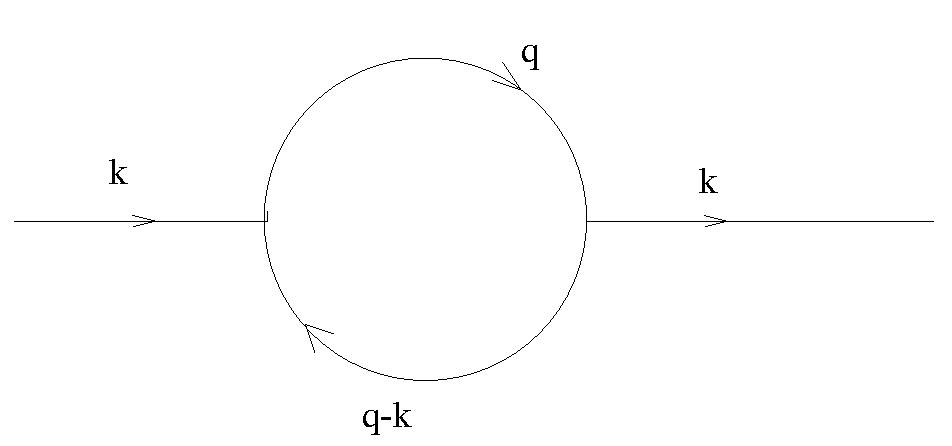
\epsfig{file=page7.eps,width=.6\linewidth}

 
 
\end{center}

So we must
put an integration parameter $q\in V^*$ on the only loop of the graph.  
Thus, the function $\Sigma_2(k^2)$ can be represented as a
single loop integral
$$
\Sigma_2(k^2)=\frac{i}{2}\int_V\frac{d^nq/(2\pi)^n}{(q^2-m^2+i\e)((q-k)^2
-m^2+i\e)}.\leqno{ 1.19}
$$
(division by 2 arises from the automorphism group of $\Gamma$, which 
has order 2).

{\bf Remark 1.} When we compute the group of automorphisms of a graph,
we do not take into account the orientation of edges. The arrows are put
on edges arbitrarily, in order to balance the momenta which are attached to 
edges. The distribution of momenta should satisfy the condition that
the sum of incoming momenta at each internal vertex should equal the sum 
of outgoing ones. 

{\bf Remark 2.} It may appear that the integral in (1.19) is real, but in fact
it is not. It is easy to see that for real negative $k^2$ the integral
is imaginary, so the r.h.s. of (1.19) is real. This happens because of 
addition of $i\e$ in the denominator. 

Now we try to compute integral (1.19). The integrand is a fraction
where the denominator is a product of two different factors. 
For a general graph, the integrand will have a product of 
many different factors 
in the denominator, which causes inconvenience. There is a remarkable trick,
which allows to convert this integral into an integral of a function
whose denominator is a power of a single factor. This trick is the ``Feynman
famous formula'':

\proclaim{Proposition 1.3} 
$$
\frac{1}{A_1...A_N}=\int_{\alpha_1+...+\alpha_N=1}\frac{1}
{(\sum \alpha_iA_i)^N}d\sigma,\leqno{ 1.20}
$$
where $d\sigma$ is a Lebesgue measure on the simplex 
with volume 1. 
\endproclaim

{\it Proof} 
We prove the statement by induction in $N$. For $N=1$, the statement 
is obvious. Let $N>1$. 

Denote the r.h.s. of (1.20) by $I_N(A_1,...,A_N)$. Then from
a homogeneity argument it follows that
$$
\int_{s\le \alpha_1+...+\alpha_N\le t}\frac{1}
{(\sum \alpha_iA_i)^N}d\alpha_1\wedge...\wedge d\alpha_N=
\frac{1}{(N-1)!}I_N(A_1,...,A_N)\ln(t/s).\leqno{ 1.21}
$$ 
Now observe that the N-form under the integral in (1.21) has the form
$d\omega$, where 
$$
\omega=\sum_{j=1}^N\frac{(-1)^{j}}{N(N-1)A_j(\sum \alpha_iA_i)^{N-1}}
d\alpha_1\wedge...\wedge \widehat{d\alpha_j}\wedge...\wedge d\alpha_N.
\leqno{ 1.22}
$$
Therefore, using Stokes' formula, we get
$$
\begin{aligned}
  &\sum_{j=1}^N \frac{1}{N(N-1)A_j} \frac{1}{(N-2)!}
  I_{N-1}(A_1,...,\hat A_j,...,A_N)\ln(t/s)\\
  &=\frac{1}{(N-1)!}I_N(A_1,...,A_N)
  \ln(t/s).
\end{aligned}
\leqno{ 1.23}
$$ 
(the integrals of $\omega$ 
over simplices $\sum\alpha_i=s,t$ cancel each other, and only the integrals
over $N$ truncated simplices remain).
Using the induction assumption, we obtain (1.20).$\square$
%\enddemo

We will use formula (1.20) for $N=2$. In this case it has the form
$$
\frac{1}{AB}=\int_0^1\frac{d\alpha}{(\alpha A+(1-\alpha)B)^2}.\leqno{ 1.24}
$$
Applying this formula to (1.19), and shifting the integration variable, 
we obtain
$$
\Sigma_2=\frac{i}{2}\int_0^1\int_V\frac{1}{(q^2+\alpha(1-\alpha)k^2-m^2+i\e)^2}
\frac{d^nq}{(2\pi)^n}d\alpha.\leqno{ 1.25}
$$

It is convenient now to perform a Wick rotation of the integration cycle.
Write any vector $q\in V$ as $(q_0,q_1)$, $q_0\in\R$, $q_1\in \R^{n-1}$,
so that $q^2=q_0^2-q_1^2$ (where $q_1^2$ is the usual squared norm). 
Consider the 1-parameter family of integration cycles, $C(t)=
\{(e^{\pi it/2}q_0,q_1)\in V_\C|(q_0,q_1)\in V\}$, 
$0\le t\le 1$. The integral (1.25) is over $C(0)$. 
It is clear that during the deformation
$C(t)$ we do not pick up any poles of the integrand in (1.25) (since $\e>0$).
Therefore, if (1.25) converges, 
the integral over $C(0)$ (which is $\Sigma_2$)
equals to the integral over $C(1)$. 

The cycle $C(1)$ is a real subspace of $V_\C$ which carries a natural
positive definite metric, $|q|^2=-q^2$. Thus, integral 
(1.25) can be written as
$$
\Sigma_2(k^2)=
\frac{i}{2}\int_0^1\int_{\R^d}\frac{1}{(|q|^2-\alpha(1-\alpha)k^2
+m^2)^2}
\frac{d^nq}{(2\pi)^n}d\alpha.\leqno{ 1.26}
$$
($i\e$ is no longer necessary, as the integrand is now smooth for negative 
$k^2$). 

It is now an exercise to compute this integral explicitly in
elementary functions. However, we are more interested in qualitative 
properties of the answer. Namely, 
from formula (1.26) it is obvious that

1) $\Sigma_2$ is analytic near $k^2=m^2$.

2) $\Sigma_2$ has a cut at the set of those values of $k^2$ for which 
the integrand is singular. 

Since the function $\alpha(1-\alpha)$ varies between $0$ and $1/4$ as
$\alpha$ varies from $0$ to $1$, the cut occurs at $k^2\ge 4m^2$. 
Thus, the function $\Sigma_2$ has the expected analytic behavior. 

{\bf Remark.} We could have considered from the very beginning a Euclidean 
theory. This means, $V$ is a Euclidean space, the Lagrangian is
$$
\int(\frac{1}{2}(\nabla\phi)^2+\frac{1}{2}m^2\phi^2+\frac{g}{3!}\phi^3)d^nx,
\leqno{ 1.27}
$$
The correlation functions are
$$
\<\phi(x)\phi(0)\>=\int_{S(V)} \phi(x)\phi(0)e^{-{\cal L}(\phi)}D\phi,\leqno{ 1.28}
$$
the propagator is $\frac{1}{k^2+m^2}$, the cubic functional corresponding to
a trivalent vertex is $-\frac{1}{3!}\delta(k_1+k_2+k_3)$, 
and the Fourier transform
of (1.28) is $\frac{1}{k^2+m^2+\Sigma}$, where $-\Sigma$ is computed as a sum 
over 1-particle irreducible connected graphs. If we try to compute $\Sigma_2$,
we will get exactly the same answer as given by (1.26), i.e.
$\Sigma_2^{\text{Euclidean}}(|k|^2)=\Sigma_2^{\text{Minkowski}}(-k^2)$. 
This is a general 
phenomenon: the Wick rotated answer for a theory in the 
Minkowski space coincides with the answer for the corresponding 
Euclidean theory. 

{\bf 1.5. Renormalization of divergent graphs.} 

Unfortunately, the integrals (1.25), (1.26) are 
divergent for $n\ge 4$, since 
the integrand does not decay rapidly enough at infinity. 
Renormalization techniques help to give meaning to these integrals anyway. 

From now until the end of the lecture we consider the case $n=4$, and the 
Euclidean picture. In this case, 
the easiest way to make sense of (1.26) is to differentiate with respect
to $k^2$. If we differentiate under the integral sign, we will obtain 
a convergent integral, and then we can integrate it back, which will define
$\Sigma_2$ up to a constant. However, this is, in general, not the best way
to proceed. The method which is usually applied in renormalization theory
is the following. 

We will replace 
the propagator
$\frac{1}{k^2+m^2}$ with a more rapidly decreasing propagator depending 
on a parameter $\L$, of the form
$P_\L=\frac{\chi(k^2,\L^2)}{k^2+m^2}$, where $\chi(k^2,\L^2)$
is a smooth function with sufficiently rapid decay
at $k^2\to \infty$ for a fixed $\Lambda$, which tends to $1$
at $\Lambda\to\infty$ (it is called 
the cutoff function). For instance, one can take
$\chi(k^2,\L^2)=\frac{\L^4}{(k^2+\L^2)^l}$, $l\in \Bbb N$.
Computing $\Sigma_2$ for this new propagator, we will obtain a convergent
integral for each finite value of $\Lambda$, and the answer 
will depend on $\Lambda$ in the following way:
$$
\Sigma_2(k^2,\L,m)= -A\ln(\Lambda/m)+O(1),\L\to\infty,\leqno{ 1.29}
$$
where $A$ is a positive constant. 
Of course, the limit of (1.29) as $\L\to\infty$
(which would be the value of (1.26)) does not exist: one says that 
the integral is logarithmically divergent. 

Now fix a constant $m=m_R>0$ (the renormalized mass). 
Given $\L$, we will adjust the mass $m_0$ of the theory
in such a way that the $\Sigma$-function 
$\Sigma(k^2,\L,m_0,g)$ for the theory with this mass and
the propagator $P_\L$ has a pole exactly at $k^2=-m_R^2$.
That is, define 
$m_0(m_R,g,\L)=m_R+O(g)$ by the equation 
$$
m_R^2=m_0^2+\Sigma(-m_R^2,\L,m_0,g).
$$
It is clear the solution of this equation (modulo $g^3$)
has the form $m_0^2=m_R^2-g^2\Sigma_2(-m_R^2,\l,m_0)$,
so by (1.29) it has the form 
$m_R^2+g^2A\ln(C\L/m_R)$, where $C$ is a constant which
depends only on the cutoff function $\chi$. 
It is easy to see that there exists a limit
$$
\Sigma_2^R(k^2,m_R,g)=\lim_{\L\to\infty}\Sigma(k^2,\L,m_0(m_R,g,\L),g).
$$
This limit is called the renormalized $\Sigma$-function.
 Of course, it depends on the choice of $m_R$. 

Let us now understand what this renormalization does  
to the Feynman diagram expansion. 
The new Lagrangian of the theory, with the 
mass $m_0$, differs from the old one (with mass $m=m_R$) by the 
additional quadratic term 
$\frac{1}{2}Ag^2\ln(C\L/m_R)\phi^2$. Therefore, according to the rules 
of Feynman calculus, the $g^2$-term of the perturbation expansion will now be 
the sum of terms corresponding to two Feynman diagrams:

\begin{center} 
 
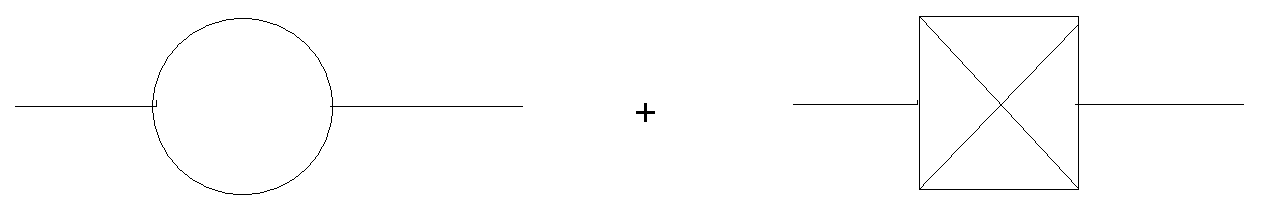
\epsfig{file=page10-1.eps,width=.7\linewidth}

 
 
\end{center}


At the 2-valent vertex of the second diagram, we put 
the tensor \[ -Ag^2\ln(C\L/m_R)\delta(k_1-k_2).\] 
This gives us an extra constant
summand in $\Sigma_2(k^2,\L,m_0)$, which compensates 
the divergence and ensures that there exists a limit 
$\Sigma_2^R$ of \[ \Sigma_2(k^2,\L,m_0(m_R,g,\L))\] as $\L\to\infty$. 
  
{\bf Remark.} We have chosen our renormalization in such a way that
the function $w(k^2)$ (modulo $g^3$) has a pole at $k^2=-m_R^2$. 
This is the reason that the constant $m_R$ is called the renormalized mass.  

{\bf 1.6. Renormalization in higher orders.}

Now let us consider the terms our Feynman diagrams expansion which 
come with a power of $g$ higher than 2. For example, consider the 
following graph,


\begin{center} 
 
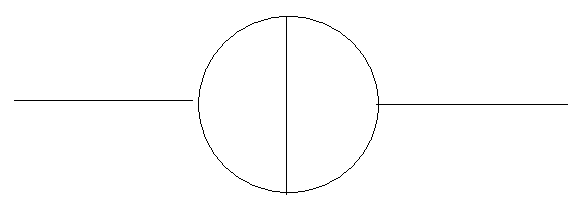
\epsfig{file=page10-2.eps,width=.4\linewidth}


\end{center}



\noindent
which occurs with $g^4$. It is easy to see that this graph defines a 
convergent integral for $n=4$. 
We will see that this is also the case for more complicated 
graphs. Namely, for $n=4$, the more vertices a graph has, the 
better is the rate of convergence of the corresponding integral.

Let us analyse the situation for arbitrary $n$. It is convenient 
to introduce the following definitions.

\proclaim{Definition 1} The superficial divergence index $div(\Gamma)$ 
of a graph $\Gamma$
is the difference of the degrees of the numerator and denominator
in the integrand of the corresponding integral. 
\endproclaim

{\bf Remark.} By the definition, the degree of the integration
variables $q_i$ and their differentials $dq_i$ equals $1$.  

\proclaim{Definition 2} A graph is called superficially divergent
if $div(\Gamma)\ge 0$ and superficially convergent if $div(\Gamma)<0$.
\endproclaim

{\bf Remark.} $\Gamma$ is called logarithmically, linearly, quadratically,...
divergent if $div(\Gamma)=0,1,2,...$.

\proclaim{Proposition 1.4} In the $\phi^3$-theory, 
$div(\Gamma)=(n-6)b_1+6-2E$, where $b_1$ is the number of 
loops, and $E$ the number of external vertices.
\endproclaim

{\it Proof} Let $M$ be the number of internal edges, 
and $N$ the number of external vertices. 
Since $\Gamma$ is connected and has only trivalent
internal vertices, we have $M=\frac{3N-E}{2}$, $b_1=\frac{N+2-E}{2}$.
It is easy to see that the degree of the numerator in the integral
corresponding to $\Gamma$ is $nb_1$ ($b_1$ loop integrations over $\R^n$), 
and the degree of the denominator is $2M$ ($M$ quadratic factors).
Thus, $div(\Gamma)=nb_1-2M=(n-6)b_1+6-2E$. 
%\enddemo

Proposition 1.4 implies the following.

1) If $n>6$, divergence worsens as the number of vertices grow. 

2) If $n=6$, all graphs with $E=2,3$ 
are equally bad (have $div(\Gamma)=6-2E$), while for $E\ge 4$ they are 
superficially convergent.

3) For $n\le 3$, all graphs with $E\ge 2$ are superficially convergent.  
 
4)   For $n=4$, the only superficially divergent graph with $E\ge 2$ is
$\Gamma_2$:

\hfill

\begin{center} 

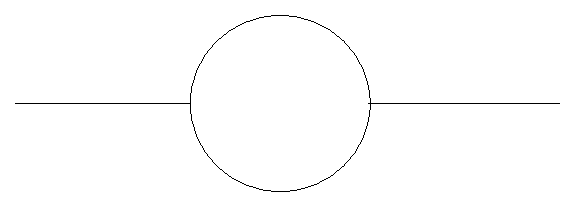
\epsfig{file=page11-1.eps,width=.4\linewidth}
 
\end{center}

\hfill


5) For $n=5$, there are finitely
many superficially divergent graphs.  
 
It is clear that superficial convergence of a graph is necessary
but not sufficient for convergence of the corresponding integral. 
Indeed, a superficially convegent integral may have a subintegral
that diverges. However, one can formulate a sufficient condition for actual
convergence in terms of superficial convergence. This condition is given 
by Weinberg theorem. 

\proclaim{Weinberg theorem} Let $\Gamma$ be a graph such that the integral
of the corresponding function over any subset of the set of loops of $\Gamma$
is superficially convergent. Then the integral corresponding to $\Gamma$
is convergent. 
\endproclaim

Weinberg theorem gaurantees that in the $\phi^3$-theory all integrals 
are convergent for $n\le 3$. Let us see what happens if $n=4$. 
In this case, we have one superficially divergent graph $\Gamma_2$.
Of course, there are infinitely many superficially convergent but still
divergent graphs, namely, all graphs which contain $\Gamma_2$ as a 
subgraph, e.g.

\begin{center} 

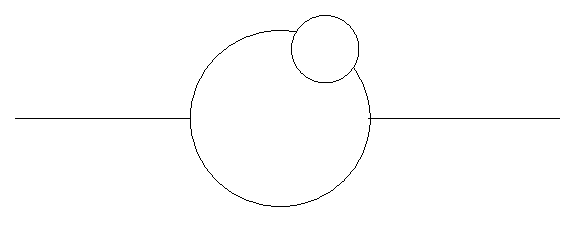
\epsfig{file=page11-2.eps,width=.4\linewidth}
 
\end{center}


However, we have renormalized the graph $\Gamma_2$, i.e. compensated 
its divergence by adding another auxiliary graph of the form

\hfill

\begin{center} 

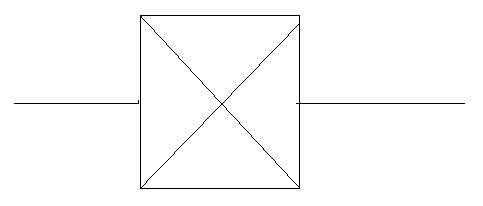
\epsfig{file=page11-3.eps,width=.4\linewidth}
 
\end{center}

\hfill

As a result, all graphs which are divergent because they contain $\Gamma_2$
will be renormalized automatically and become convergent. That is, the divergence of each graph containing $\Gamma_2$ will  be compensated by
a counterterm, in which $\Gamma_2$ will be replaced by the above auxiliary
graph. The fact that this ensures convergence in all orders follows from
the ``Strong Weinberg theorem'', which states, roughly, that if all graphs 
at orders $\le N$ (in $g$) have been renormalized, then all superficially
convergent graphs at order $N+1$ are actually convergent. 
Thus, after mass renormalization all correlation functions
become well defined. 

{\bf Remark.} As we explain above, the procedure of setting the 1-point 
function to zero in $\phi^3$-theory also requires renormalization. 
Namely, we have two graphs with one external vertex,
\begin{center} 

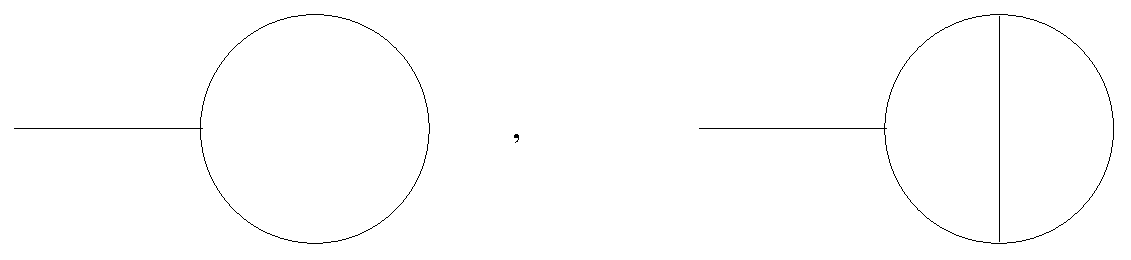
\epsfig{file=page11-4.eps,width=.8\linewidth}
 
\end{center}

\noindent
among which the first is quadratically divergent and the second 
logarithmically. Consider a new Lagrangian of the form
${\cal L}'={\cal L}+B(m,g,\L)\int \phi$, where $B(m,g,\L)=
a(m,g)\L^2+b(m,g)\L+c(m,g)\ln(\L/m)+d(m,g)$, and choose the constants
$a,b,c,d$ in such a way that the limit of the 1-point function
for this Lagrangian, computed for
the cutoff propagator at $\L$, tends to $0$.
The constants $a,b,c,d$ are determined by this condition uniquely, but 
they of course depend on the cutoff function $\chi$. In the language of 
Feynman graphs, this corresponds to compensating the divergence 
in the sum
\begin{center} 

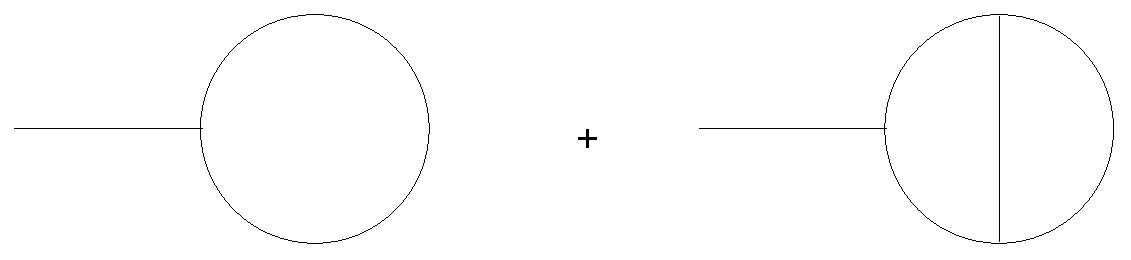
\epsfig{file=page11-5.eps,width=.8\linewidth}
 
\end{center}

\noindent
by adding a third summand

\hfill

\begin{center} 

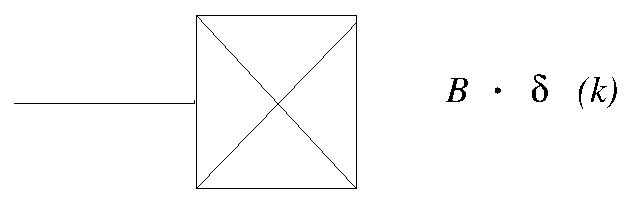
\epsfig{file=page15.eps,width=.4\linewidth}
 
\end{center}

\hfill

where at the vertex we put the linear functional $B\cdot \delta(k)$. 
This reduces the problem of renormalization of the $\phi^3$ theory 
to renormalization of the graph $\Gamma_2$, which was done above. 

\end{document}  


